
\section{Auswertung}
\subsection{Zählrohr-Charakteristik}
\begin{table}
\centering
\caption{Gemessene Werte für die Spannung, Zählrate und den Strom}
\label{tab:werte}
\begin{tabular}{c c c}
\toprule
{U/V} & {N/$\mathrm{\frac{1}{min}}$} & {$\bar{I}\,/\, \mathrm{\mu A}$}\\
\midrule
310 & 12443 & 0,2\\
310 & 13282 & 0,2\\
330 & 13400 & 0,2\\
340 & 13647 & 0,2\\
350 & 13371 & 0,2\\
360 & 13655 & 0,2\\
370 & 13613 & 0,2\\
380 & 13671 & 0,3\\
390 & 13910 & 0,3\\
400 & 13659 & 0,4\\
410 & 13686 & 0,4\\
420 & 13894 & 0,4\\
430 & 13783 & 0,4\\
440 & 14058 & 0,4\\
450 & 13954 & 0,5\\
460 & 13752 & 0,6\\
470 & 13802 & 0,6\\
480 & 13659 & 0,6\\
490 & 13907 & 0,6\\
500 & 13858 & 0,6\\
510 & 14033 & 0,7\\
520 & 13722 & 0,7\\
530 & 13912 & 0,8\\
540 & 13872 & 0,8\\
550 & 14125 & 0,8\\
560 & 14188 & 0,8\\
570 & 14223 & 0,8\\
580 & 14231 & 0,8\\
590 & 13926 & 0,9\\
600 & 14324 & 0,9\\
610 & 14042 & 1,0\\
620 & 14326 & 1,0\\
630 & 14142 & 1,0\\
640 & 14380 & 1,0\\
650 & 14367 & 1,1\\
660 & 14553 & 1,1\\
670 & 14578 & 1,2\\
680 & 14745 & 1,2\\
690 & 14741 & 1,2\\
700 & 14802 & 1,2\\
\bottomrule
\end{tabular}
\end{table}

In Abbildung \ref{fig:char} sind die im Versuch gemessenen Werte aufgetragen.
Die Werte für die Zählrate wurden aus Tabelle \ref{tab:werte} entnommen
und dafür durch die Messzeit von 60\,s geteilt.
Die Fehler ergeben sich durch $\sqrt{N}/60$.\\
\begin{figure}
  \centering
  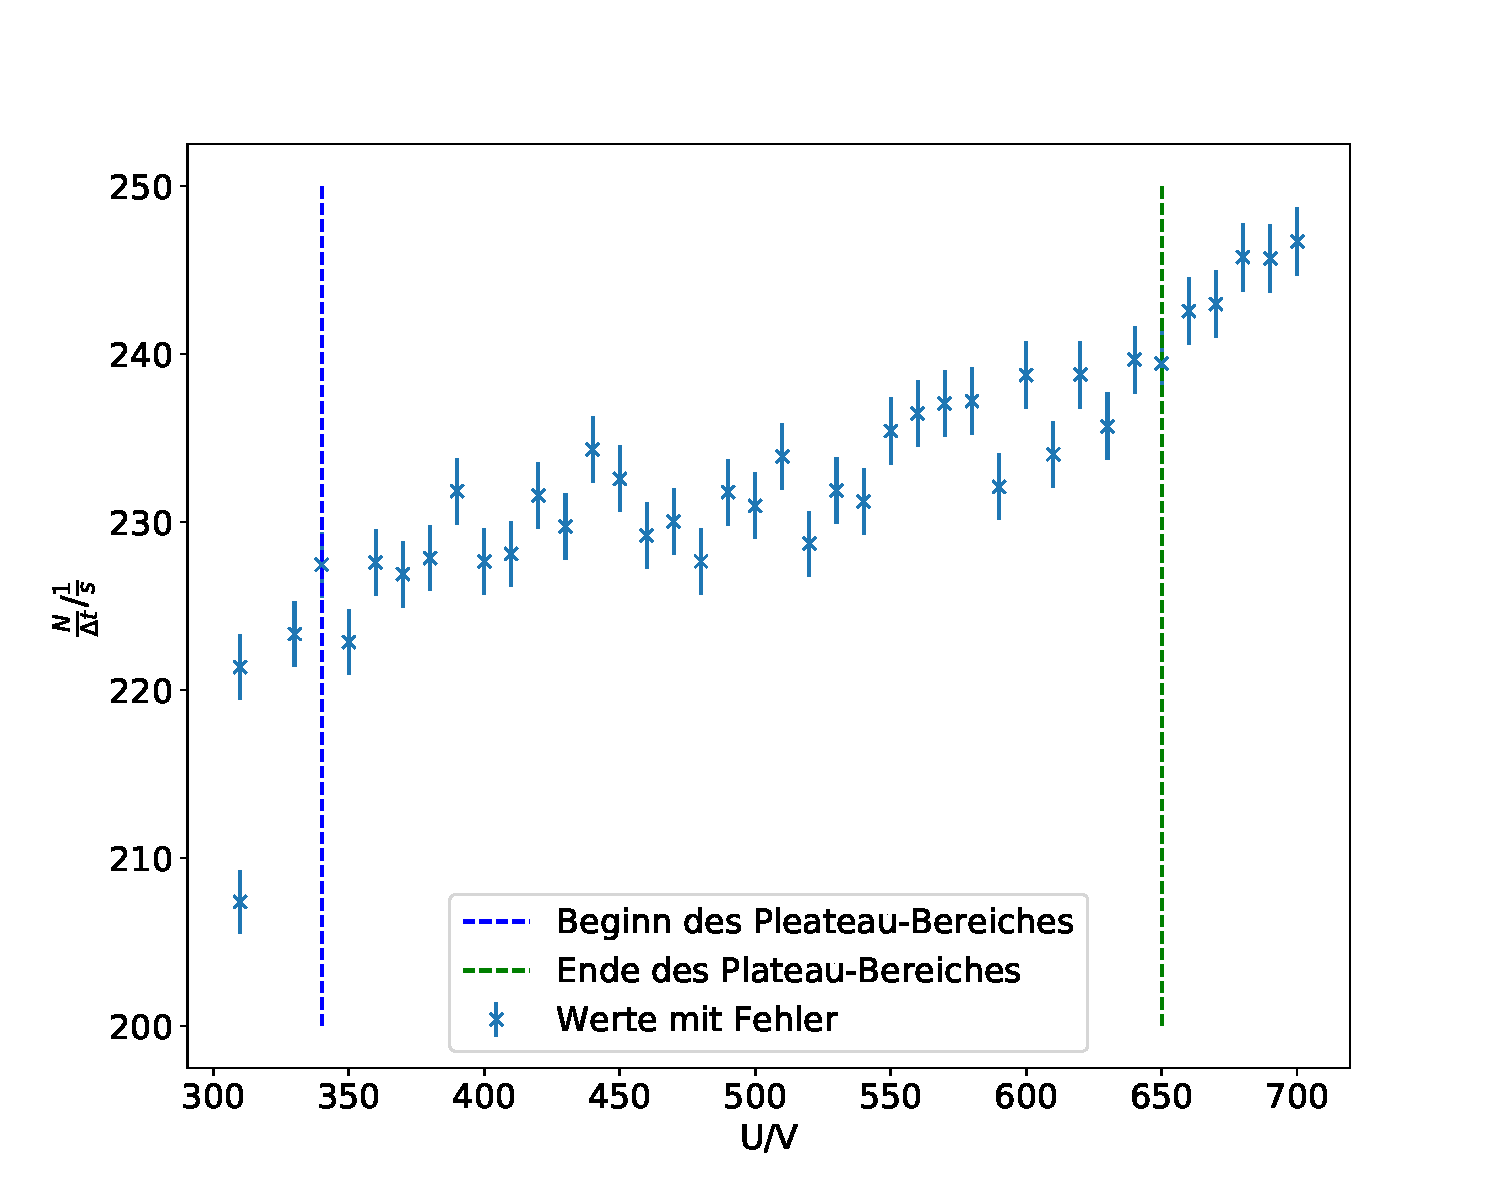
\includegraphics[scale=0.7]{plateau.pdf}
  \caption{Charakteristik des Geiger-Müller-Zählrohrs}
  \label{fig:char}
\end{figure}
Der Begin und das Ende des Plateau-Bereiches wurde aus den Messwerten entnommen.
Das Plateau liegt in dem Bereich von 340\,V bis 650\,V.\\
In Abbildung \ref{fig:plateau} ist der Plateau-Bereich aufgetragen und es wurde eine lineare Regression mit
\begin{equation*}
\frac{N}{\Delta t} = a\cdot U + b
\end{equation*}
Dabei ist N die Zählrate pro 60\,s.
\begin{figure}
  \centering
  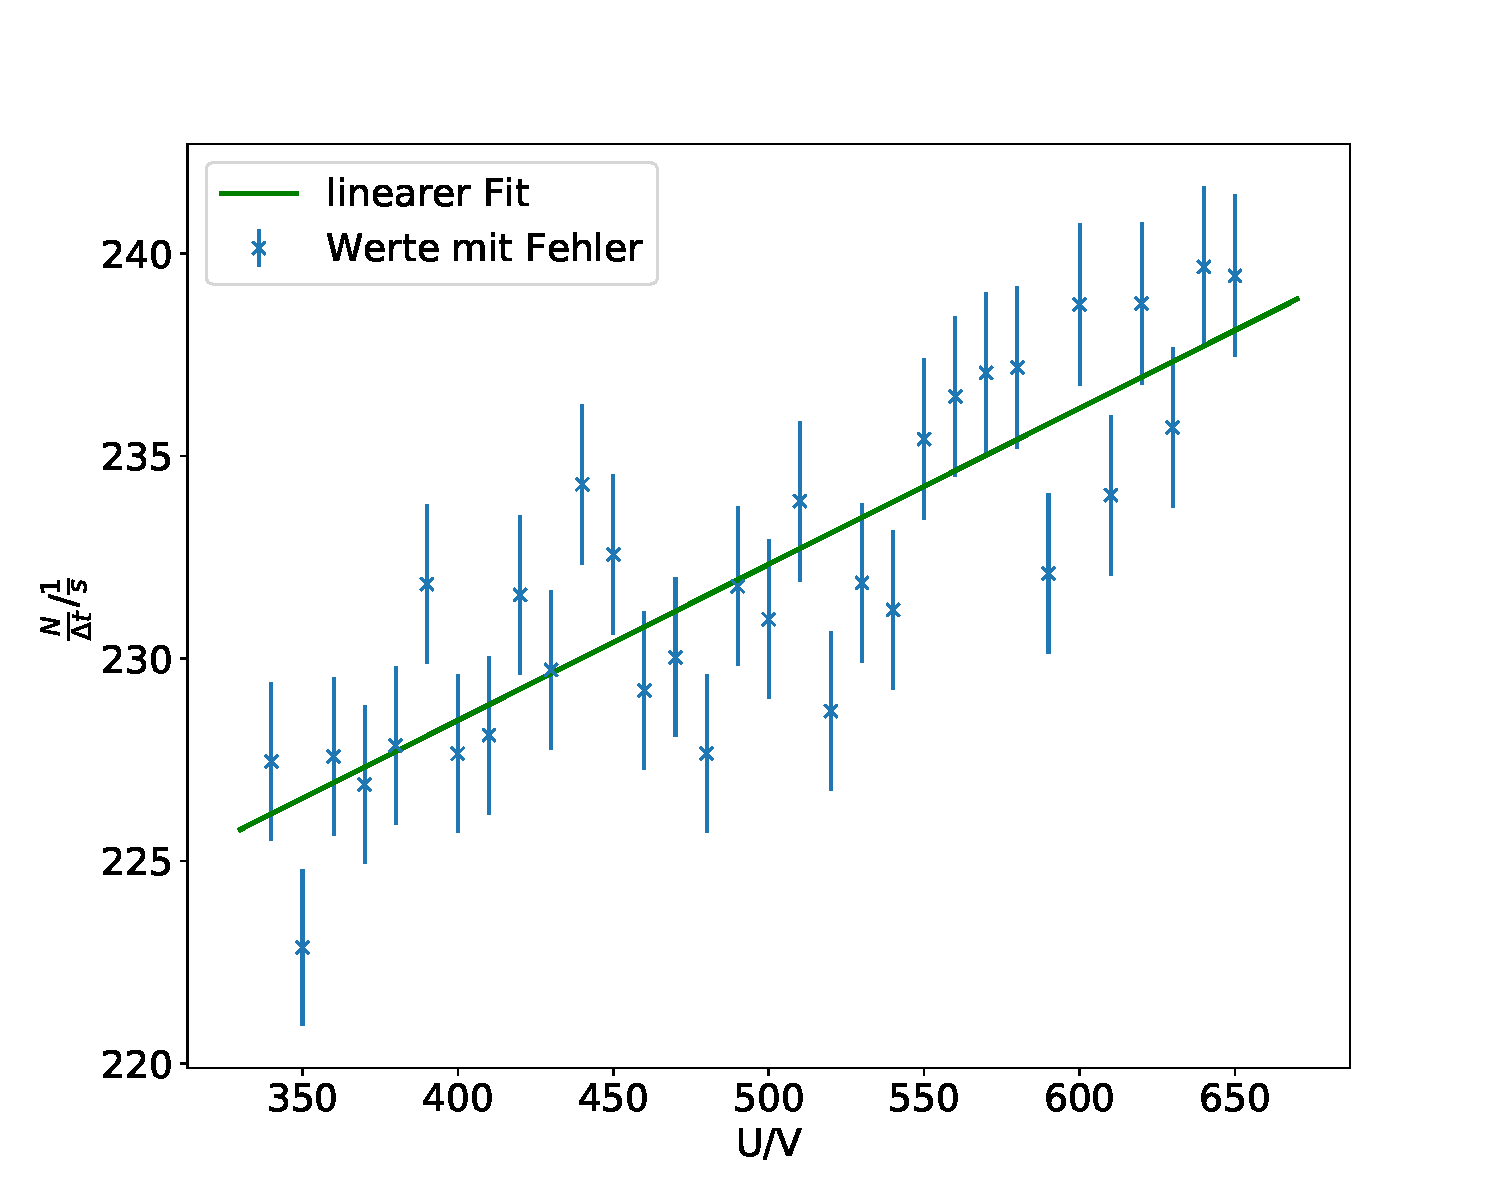
\includegraphics[scale=0.7]{plateau2.pdf}
  \caption{Plateau mit linearer Regression}
  \label{fig:plateau}
\end{figure}
Die Parameter der Regression lauten:
\begin{align*}
  a &= (0,039\pm 0,004)\,\mathrm{\frac{1}{Vs}}\\
  b &= (213,1 \pm 2,2)\, \mathrm{\frac{1}{s}}
\end{align*}
In Prozent entspricht das einer Steigung von (1,7\pm1,8)\,\%. %Nochmal nachgucken!!!

%primär und Nachentladungsimpulsen!!

\subsection{Messung der Totzeit mit zwei unterschiedlichen Methoden}
\subsubsection{Bestimmung mit Hilfe des Oszillographen}

Zunächst wird die Totzeitbestimmung über den Oszillographen durchgeführt.
Die Werte sind in Tabelle \ref{tab:tez} zu finden.
\begin{table}
\centering
\caption{Totzeit und Erholungszeit}
\label{tab:tez}
\begin{tabular}{c c c}
\toprule
{U/V} & {Totzeit/$\mathrm{\mu s}$} & {Erholungszeit/$\mathrm{ms}$}\\
\midrule
500 & 200 & 0,86 \\
520 & 210 & 1,28 \\
540 & 230 & 1,08 \\
\bottomrule
\end{tabular}
\end{table}

Die Totzeit hat somit einen Wert von
\begin{equation*}
  T = (2,13\pm0,09)\cdot 10^{-4}\,\mathrm{s}
\end{equation*}
Die Erholungszeit wird ebenfalls mi den Werten aus Tabelle \ref{tab:tez} bestimmt und hat einen Wert von
\begin{equation*}
  E_z = (1,073 \pm 0,121)\,\mathrm{ms}
\end{equation*}
Die Formel für die Standartabweichung lautet
\begin{equation*}
 \sigma_{T, E_z} =   \frac{1}{\sqrt{3}}\sqrt{\frac{1}{2}\cdot\sum\left(x_{T, E_z}-\bar{x}_{T, E_z}\right)^2}
\end{equation*}
Der Mittelwert berechnet sich mit
\begin{equation*}
  \bar{x}_{T, E_z} = \frac{1}{3}\cdot \sum x_{T, E_z}
\end{equation*}


\subsubsection{Bestimmung mit der zwei-Quellen-Methode}
Für diese Methode wurden zunächst die Zählraten $N_1$, $N_2$ und $N_{1+2}$ aufgenommen.
Die Werte sind in Tabelle \ref{tab:zähl} aufgelistet.
\begin{table}
\centering
\caption{Totzeit und Erholungszeit}
\label{tab:zähl}
\begin{tabular}{c c c c}
\toprule
{} & {N/$\mathrm{\frac{1}{min}}$} & {N/$\mathrm{\frac{1}{s}}$} & {$\Delta N$}\\
\midrule
 $N_1$    & 13703 & 228,38  & 1,95 \\
$N_2$     & 17646 & 294,10  & 2,21 \\
$N_{1+2}$ & 30720 & 512,00   & 2,92 \\
\bottomrule
\end{tabular}
\end{table}
Die Bedingung
\begin{equation*}
  N_{1+2} < N_1 + N_2
\end{equation*}
ist somit erfüllt.
Die Totzeit T kann nährungsweise geschrieben werden als
\begin{equation*}
  T \approx  \frac{N_1 +N_2 -N_{1+2}}{2N_1N_2}
\end{equation*}
\begin{equation*}
  T \approx (7,8\pm 3,4)\cdot 10^{-5} \, \mathrm{s}
\end{equation*}
Der Fehler berechnet sich mit
\begin{equation*}
  \sigma T = \sqrt{\left(\frac{-N_1^2+N_2N_{1+2}}{2N_1^2N_2^2}\cdot\sigma_{N_2}\right)^2+
  \left(\frac{-N_2^2+N_1N_{1+2}}{2N_1^2N_2^2}\cdot\sigma_{N_1}\right)^2+
  \left(-\frac{1}{2N_1N_2}\cdot\sigma_{N_{1+2}}\right)^2}
\end{equation*}

\subsection{Bestimmung der pro Teilchen vom Zählrohr freigesetzten Ladungsmenge }

Um die Ladungsmenge bestimmen zu können werden die Werte für den mittleren Zählerstrom benötigt.
Diese werden aus Tabelle \ref{tab:werte} entnommen.
Die Ladungsmenge besttimmt sich mit Formel:
\begin{align*}
  \bar{I} &= \frac{\Delta Q}{\Delta t}\cdot Z \\
  \Delta{Q} &= \frac{\bar{I}\cdot \Delta t}{Z}
\end{align*}

Z ist die Teilchenzahl.
$\Delta Q$ ist die Transportierte Ladungsmenge pro $\Delta t = 60\,s$

Die Ergebnisse sind in Tabelle \ref{tab:Q} dargestellt.
Der Fehler berechnet sich mit Formel:
\begin{equation*}
  \sigma Q =  I \cdot \left(\frac{\Delta t}{Z}\right)^2\cdot \frac{\sqrt{Z}}{\Delta t}
\end{equation*}

\begin{table}
\centering
\caption{Freigesetzte Ladungsmenge}
\label{tab:Q}
\begin{tabular}{c c c c }
\toprule
{U/V} & {N/$\mathrm{\frac{1}{min}}$} & {$\bar{I}\,/\, \mathrm{\mu A}$}  & {$\frac{\Delta Q}{e_0}\cdot 10^9$}\\
\midrule
310 & 12443 & 0,2 & $(6,019\pm 0,054)$ \\
310 & 13282 & 0,2 & $(5,639\pm 0,049)$\\
330 & 13400 & 0,2 & $(5,589\pm 0,048)$\\
340 & 13647 & 0,2 & $(5,488\pm 0,047)$\\
350 & 13371 & 0,2 & $(5,602\pm 0,048)$ \\
360 & 13655 & 0,2 & $(5,485\pm 0,047)$\\
370 & 13613 & 0,2 & $(5,502\pm 0,047)$ \\
380 & 13671 & 0,3 & $(8,218\pm 0,070)$  \\
390 & 13910 & 0,3 & $(8,077\pm 0,068)$ \\
400 & 13659 & 0,4 & $(10,967\pm 0,094)$ \\
410 & 13686 & 0,4 & $(10,945\pm 0,094)$ \\
420 & 13894 & 0,4 & $(10,781\pm 0,091)$ \\
430 & 13783 & 0,4 & $(10,868\pm 0,093)$ \\
440 & 14058 & 0,4 & $(10,656\pm 0,090)$ \\
450 & 13954 & 0,5 & $(13,419\pm 0,114)$ \\
460 & 13752 & 0,6 & $(16,339\pm 0,140)$ \\
470 & 13802 & 0,6 & $(16,280\pm 0,140)$ \\
480 & 13659 & 0,6 & $(16,450\pm 0,141)$ \\
490 & 13907 & 0,6 & $(16,157\pm 0,137)$\\
500 & 13858 & 0,6 & $(16,214\pm 0,138)$ \\
510 & 14033 & 0,7 & $(18,680\pm 0,158)$ \\
520 & 13722 & 0,7 & $(19,104\pm 0,163)$ \\
530 & 13912 & 0,8 & $(21,535\pm 0,183)$ \\
540 & 13872 & 0,8 & $(21,597\pm 0,183)$ \\
550 & 14125 & 0,8 & $(21,210\pm 0,178)$ \\
560 & 14188 & 0,8 & $(21,116\pm 0,177)$ \\
570 & 14223 & 0,8 & $(21,064\pm 0,177)$ \\
580 & 14231 & 0,8 & $(21,052\pm 0,176)$ \\
590 & 13926 & 0,9 & $(24,202\pm 0,205)$ \\
600 & 14324 & 0,9 & $(23,530\pm 0,197)$ \\
610 & 14042 & 1,0 & $(26,669\pm 0,225)$ \\
620 & 14326 & 1,0 & $(26,141\pm 0,218)$ \\
630 & 14142 & 1,0 & $(26,481\pm 0,223)$ \\
640 & 14380 & 1,0 & $(26,042\pm 0,217)$ \\
650 & 14367 & 1,1 & $(28,673\pm 0,239)$ \\
660 & 14553 & 1,1 & $(28,306\pm 0,235)$ \\
670 & 14578 & 1,2 & $(30,826\pm 0,255)$ \\
680 & 14745 & 1,2 & $(30,477\pm 0,251)$  \\
690 & 14741 & 1,2 & $(30,486\pm 0,251)$ \\
700 & 14802 & 1,2 & $(30,360\pm 0,250)$ \\
\bottomrule
\end{tabular}
\end{table}

\section{Diskussion}
Im ersten Versuchsteil wurde die Charakteristik des Zählrohres bestimmt.
Die Parameter für die durchgeführte Regression weisen nur geringe Fehler auf.
Die Merkmale eines Geiger-Müller-Zählrohrs sind im großen und ganzen zu erkennen.
Lediglich der zu erwartende exponentielle Anstieg nach Ende des Plateau-Bereiches ist nicht genau heraus zu sehen.

Die Bestimmung der Totzeit wurde mit Zwei Methoden durchgeführt.
Die beiden Ergebnisse für die Totzeit lauten:
\begin{align*}
  T &= (2,13\pm0,08)\cdot 10^{-4}\,\mathrm{s}\\
  T &= (7,8\pm 3.4)\cdot 10^{-5} \, \mathrm{s}
\end{align*}
Der große Unterschied zwischen den beiden Werten ist mit der Messsmethode mit Hilfe des Oszillographen zu erklären.
Diese ist sehr ungenau, da der Wert sehr stark schwankte.

Die Ergebnisse für die freigesetze Ladung sind, wie in Abbildung \ref{fig:Bereiche} zu sehen, in der zu erwartenden Größenordnung,
sodass davon ausgegangen werden kann, dass keine größeren Fehler gemacht wurden.
